% Created 2022-09-07 Wed 08:43
% Intended LaTeX compiler: pdflatex
\documentclass[bigger]{beamer}
\usepackage[utf8]{inputenc}
\usepackage[T1]{fontenc}
\usepackage{graphicx}
\usepackage{grffile}
\usepackage{longtable}
\usepackage{wrapfig}
\usepackage{rotating}
\usepackage[normalem]{ulem}
\usepackage{amsmath}
\usepackage{textcomp}
\usepackage{amssymb}
\usepackage{capt-of}
\usepackage{hyperref}
\usetheme[progressbar=foot]{metropolis}
\author{Edmund Miller}
\date{2022-09-07 Wed}
\title{Nascent Transcript Identification}
\hypersetup{
 pdfauthor={Edmund Miller},
 pdftitle={Nascent Transcript Identification},
 pdfkeywords={},
 pdfsubject={},
 pdfcreator={Emacs 29.0.50 (Org mode 9.6)}, 
 pdflang={English}}
\usepackage{biblatex}
\addbibresource{~/sync/reference/bibliography.bib}
\addbibresource{~/sync/reference/biochemistry.bib}
\addbibresource{~/sync/reference/genomics.bib}
\addbibresource{~/sync/reference/molecular_biology.bib}
\addbibresource{~/sync/reference/molecular_biology_project.bib}
\addbibresource{~/sync/reference/nascent_pipeline.bib}
\addbibresource{~/sync/reference/viralintegration.bib}
\addbibresource{~/sync/reference/books.bib}
\begin{document}

\maketitle


\begin{frame}[label={sec:orgba95986},fragile]{groHMM fix}
 \begin{itemize}
\item Failed whenever we ran on full datasets
\item Sruthi fixed it by adding \texttt{keepStandardChromosomes}
\item I expect this to have issues with CHM13
\end{itemize}
\end{frame}
\section*{CHM13 Struggles}
\label{sec:org3b7bc68}
\begin{frame}[label={sec:org37eea3a}]{CHM13 Struggles}
\begin{itemize}
\item v2.0 has been released
\item genbank chr aliases are used by default
\end{itemize}
\begin{center}
\begin{tabular}{lllll}
genbank & refseq & assembly & ncbi & ucsc\\
\hline
CP068255.2 & NC$\backslash$\textsubscript{060947.1} & X & X & chrX\\
CP068256.2 & NC$\backslash$\textsubscript{060946.1} & 22 & 22 & chr22\\
\end{tabular}
\end{center}
\end{frame}

\begin{frame}[label={sec:orgf3b4e66}]{CHM13 Struggles}
\begin{center}
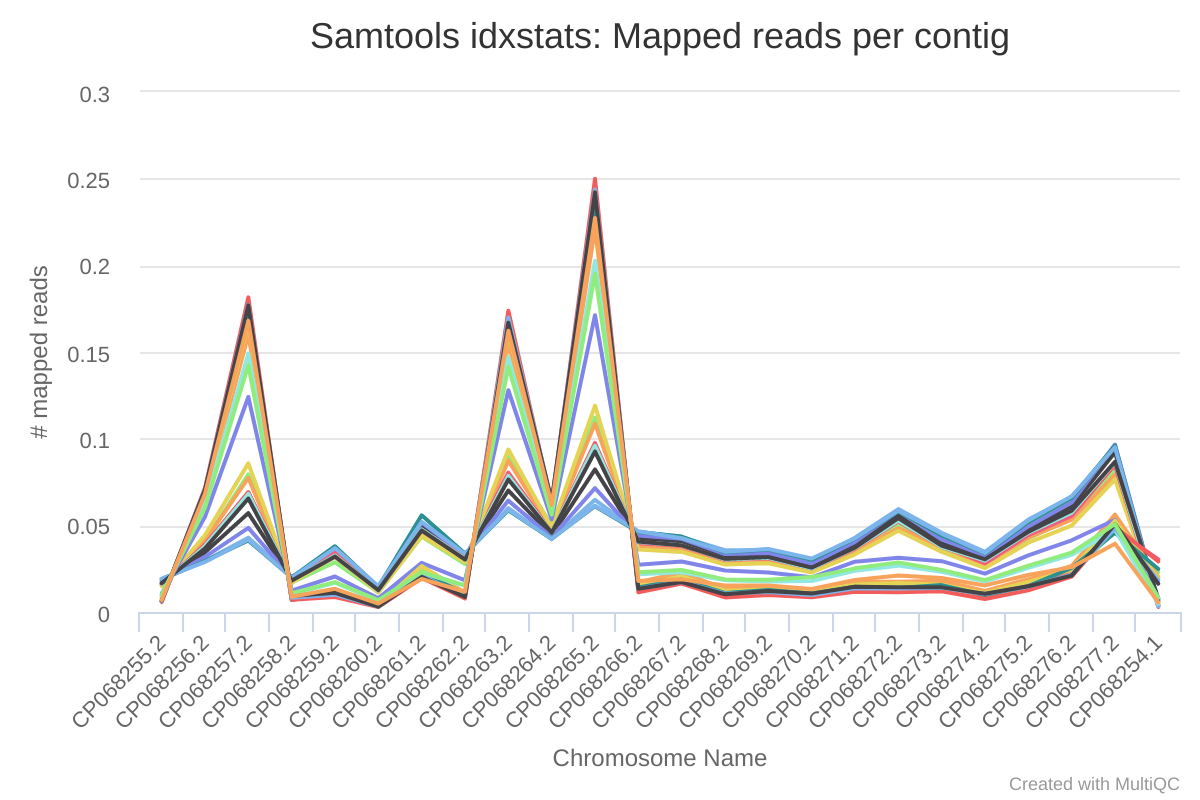
\includegraphics[width=.9\linewidth]{/home/emiller/src/personal/edmundmiller-dev/static/org-attach/99/6c3081-dce2-41c5-bccc-8de86c58e920/_20220906_220028screenshot.png}
\end{center}
\end{frame}
\begin{frame}[label={sec:org90feffd}]{CHM13 Struggles}
\begin{itemize}
\item Rebuilding indexes with refgenie
\item In process of getting them hosted to AWS igenomes for ease of use.
\end{itemize}
\end{frame}

\section*{Understanding PINTS Results}
\label{sec:org8305f42}
\begin{frame}[label={sec:org815508a}]{IOU of GENCODE (Annot.) and those predicted by different tools}
\begin{center}
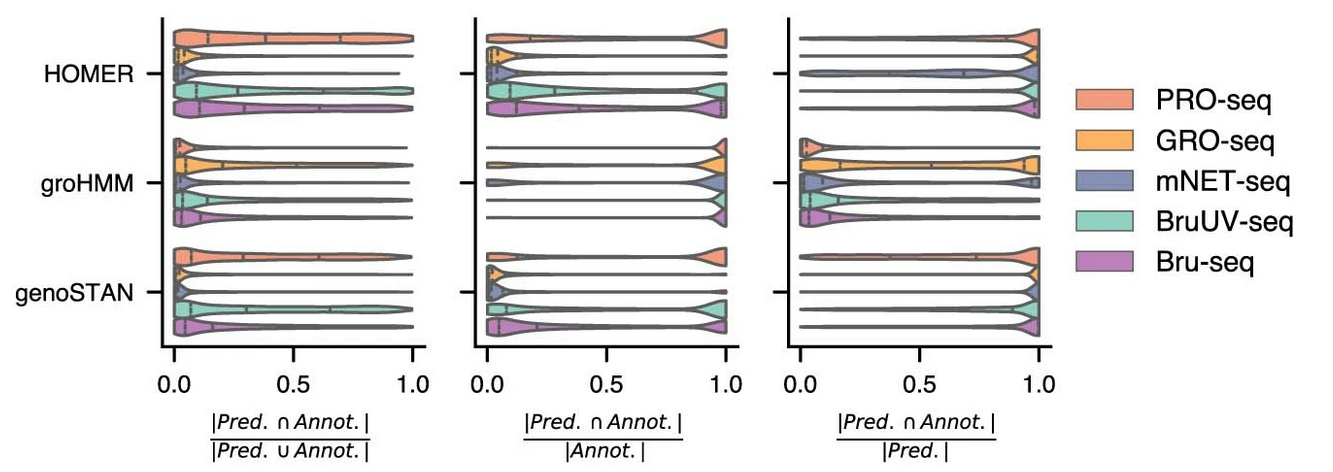
\includegraphics[width=.9\linewidth]{/home/emiller/src/personal/edmundmiller-dev/static/org-attach/dc/f0d0a6-1ba7-4b67-97e5-74b9d4ca892d/_20220907_081721screenshot.png}
\end{center}

Consistencies vary greatly between transcription units annotated
\end{frame}

\begin{frame}[label={sec:orge776468}]{Schematic plot of PINTS}
\begin{center}
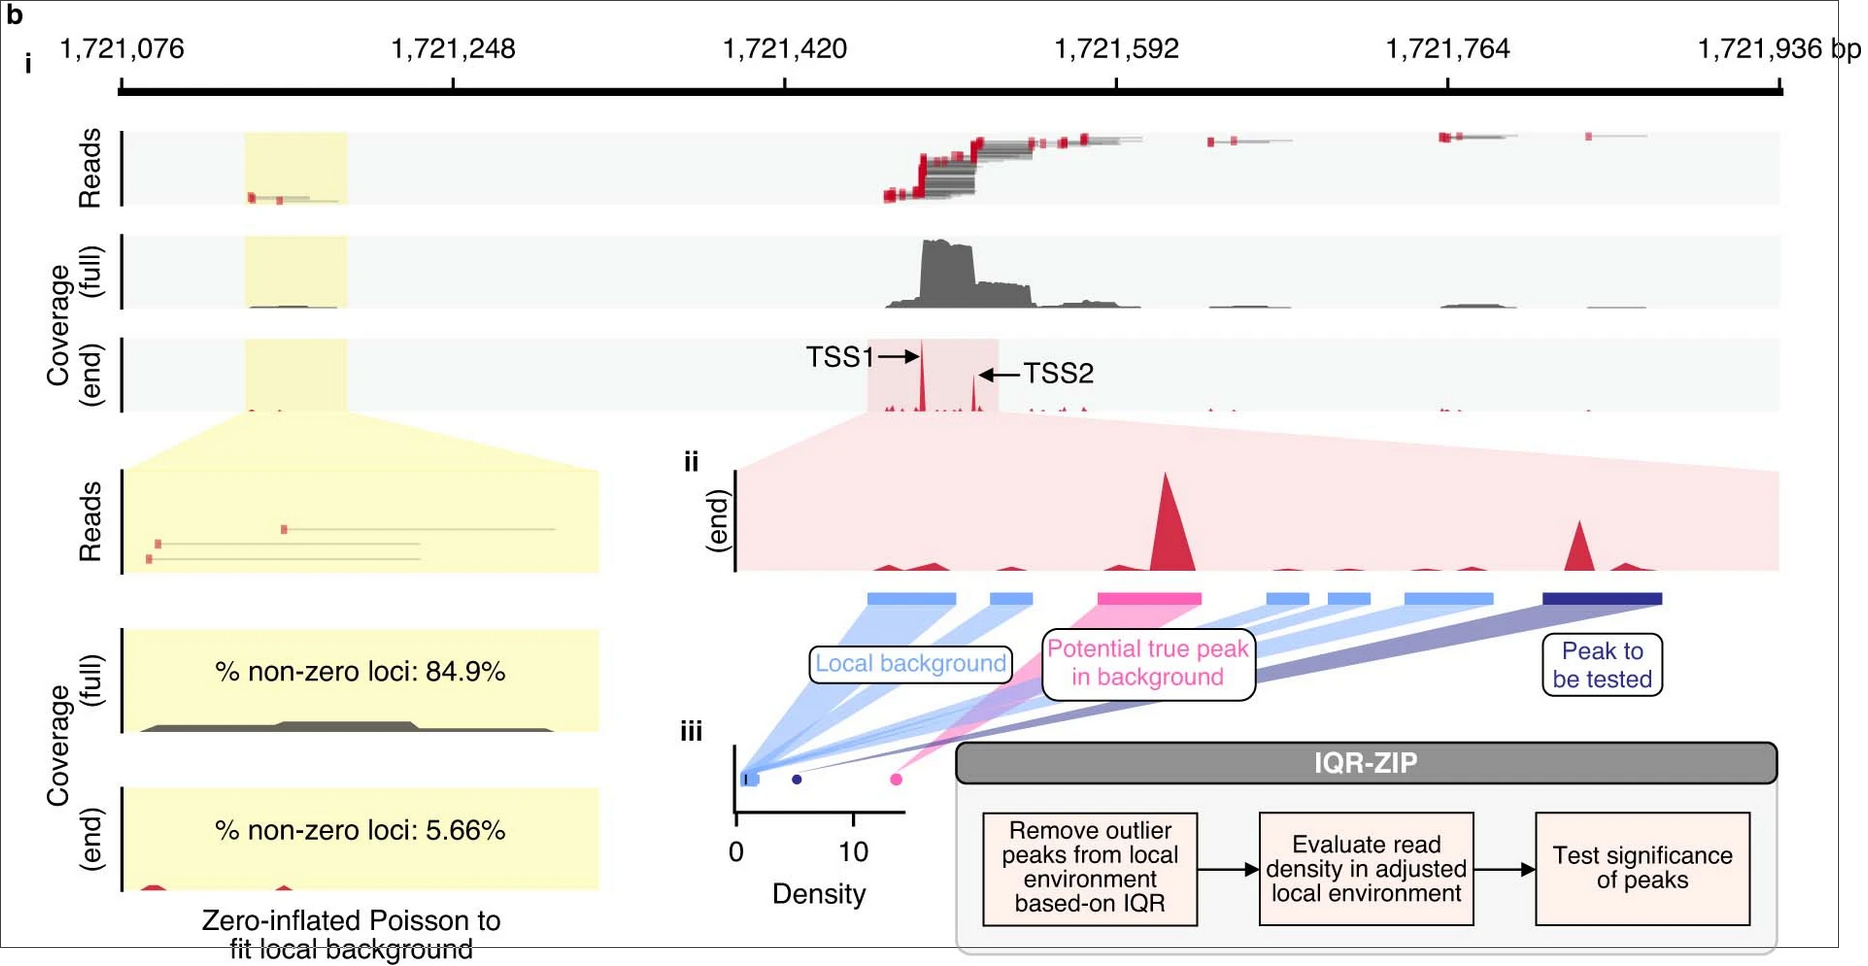
\includegraphics[width=.9\linewidth]{/home/emiller/src/personal/edmundmiller-dev/static/org-attach/52/33a535-b99a-4e1e-831e-63fa79c3e921/_20220907_082129screenshot.png}
\end{center}
\end{frame}


\begin{frame}[label={sec:org4f5bba1}]{How to count PINTS TREs?}
\begin{enumerate}
\item \uline{1 to 1 transcripts to samples}. The predicted TSS's for IMR0h would only be
counted for IMR0h, and not counted for IMR1h. \alert{One TSV per sample}
\item \uline{Transcripts are counted across all samples}. So the TSS's for IMR0h are
counted across all the samples and then combined. So you'd end up with a \alert{tsv
per sample x sample} with IMR0h TSS across all the samples, a TSV for IMR1h.
\item \uline{Combine the TSS's across all samples and count once per sample}. end up with
\alert{one TSV} with all the transcripts counts for every sample.(What happens with
homer/groHMM)
\end{enumerate}
\end{frame}

\begin{frame}[label={sec:orge94cc12}]{How to count PINTS TREs?}
\begin{quote}
For some types of analysis, such as transcript identification, it is a good idea
to create a single META-experiment that contains all of the GRO-Seq reads for a
given cell type
\end{quote}

Planning on something similar to \alert{option 3} to follow homer recommendations to
avoid missing low transcription
\end{frame}

\begin{frame}[label={sec:orgd25cb4a}]{Future action}
\begin{itemize}
\item Couple of outstanding GitHub issues on PINTS
\item Updating test dataset to have at-least a ``peak''(artificially selected)
\item Create a test dataset that uses chr 21 for sample 1 and chr 22 for sample 2
and see if there's any cross-over
\end{itemize}
\end{frame}

\section*{How do we determine 3' end?}
\label{sec:orge93ebfa}
\begin{frame}[label={sec:orgcdfe424}]{PINC}
\begin{itemize}
\item Prediction of lncRNA based on RNA-Seq data.
\item Easier problem because they can filter based off the coding-potential
\item Brought some inspiration for basic filtering for end-users
\end{itemize}
\end{frame}

\begin{frame}[label={sec:orgc4caa34}]{PINTS Issues}
\begin{itemize}
\item Are we getting just the TSS with the GROSeq setting? Or the full nascent transcript?
\item If it's just the TSS, could we combine their improved TSS identification to
filter homer or groHMM \emph{de novo} transcripts?
\end{itemize}
\end{frame}

\begin{frame}[label={sec:orgb9cd6ab}]{Homer Identification}
\begin{center}
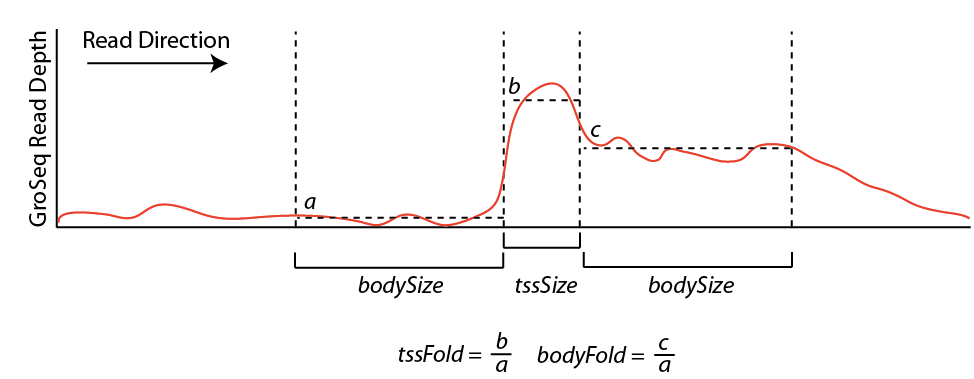
\includegraphics[width=.9\linewidth]{/home/emiller/src/personal/edmundmiller-dev/static/org-attach/a2/6ed570-97a2-4f5f-9c9c-72b5857c63d5/_20220907_071614screenshot.png}
\end{center}
\end{frame}

\begin{frame}[label={sec:org95c0dcb}]{PINTS for refining nascent transcripts}
\begin{center}
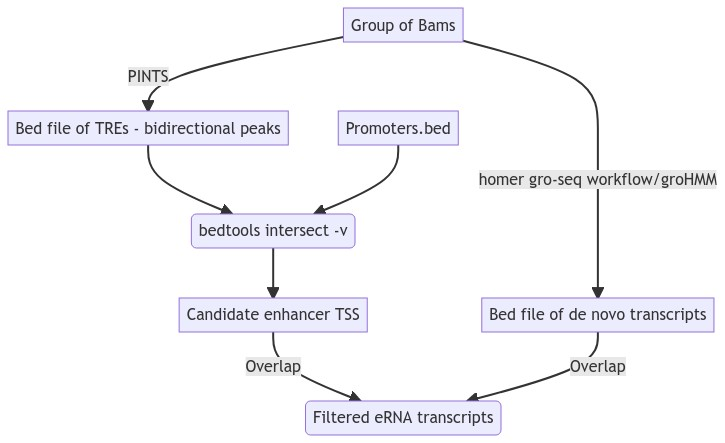
\includegraphics[width=.9\linewidth]{/home/emiller/src/personal/edmundmiller-dev/static/org-attach/6a/4a290f-4071-49dd-abdf-bfa0beaaf15d/_20220907_075231screenshot.png}
\end{center}
\end{frame}

\begin{frame}[label={sec:org5658131}]{Training a model to find 3' ends}
\begin{itemize}
\item Shayne mentioned she still does a lot of manual validation
\item Perhaps something similar Deepvariant that ``looks'' at the pileups
\end{itemize}
\end{frame}
\end{document}
